%!TEX root = ../thesis.tex
%*******************************************************************************
%****************************** Fourth Chapter *********************************
%*******************************************************************************
\chapter{Determinants of cross-tissue cell type identity and distribution} \label{chap:CT_bio}

% **************************** Define Graphics Path **************************
\ifpdf
    \graphicspath{{Chapter4/Figs/Raster/}{Chapter4/Figs/PDF/}{Chapter4/Figs/}}
\else
    \graphicspath{{Chapter4/Figs/Vector/}{Chapter4/Figs/}}
\fi
Cell identity can be defined by the genes it expresses. A continuously increasing number of studies has applied scRNA-seq to profile cells from various body locations and describe the cells that make up a tissue, in the steady-state or disease. A smaller number of studies have focused on the differences between the cell types detected in different tissues~\citep{miragaia_single-cell_2019,scott_transcription_2018}. However, we don't yet know how variable transcriptome of most cell types is between tissues, and how it relates to the tissue transcriptome.

This Chapter outlines the construction of a human cell type reference based on single-cell transcriptomics, by applying the \textit{CellTypist} framework presented in Chapter~\ref{chap:CT_method}. It will be demonstrated how this reference can be used for automatic classification of newly generated data and discuss its current advantages and limitations. The present Chapter will also focus on the interpretability of this pipeline, and reveal the genes driving cell identity across tissues. We will further dissect the relationships across tissues established by \textit{CellTypist}, and explore the influence of different cell types in tissue biology.

The work presented in this Chapter was partly developed with the assistance of Ni Huang, who contributed to the collection and integration of published datasets. The analyses here performed are based on the methodology outlined in Chapter~\ref{chap:CT_method}. Supplementary figures are included in Appendix~\ref{appendix:CTsub}.


\section{Introduction}
\label{section4.1}




\section{Results}
\label{section4.2}
\subsection{Human data collection and organisation}
\label{section4.2_coll}
To obtain a global, cross-tissue perspective of human cell types, we obtained a broad representation of single-cell transcriptomes with by collecting several publicly available scRNA-seq datasets (Table~\ref{table:tab_4_1}). Information about tissue, scRNA-seq protocol, sampling method, and cell type annotation (when available) were obtained from the respective publications and data repositories, together with the gene expression matrices.

% table: Dataset; number of cells; ref
\begin{table}[ht!] % p for putting it in the next page available
\footnotesize
\caption[Datasets collected and references]{Datasets collected and references}
\centering
\label{table:tab_4_1}

\begin{tabular}{l|c|r}
\toprule
~\textbf{Dataset} & ~\textbf{Reference} & ~\textbf{\# cells} \\
\midrule
baron16 & ~\citep{baron_single-cell_2016} & 8.569  \\

bjorklund16 & ~\citep{bjorklund_heterogeneity_2016} & 648  \\

gierahn17 & ~\citep{gierahn_seq-well:_2017} & 3.694  \\

guo18 & ~\citep{guo_adult_2018} & 12.053  \\

habib17 & ~\citep{habib_massively_2017} & 14.963  \\

hcaImmune18 & \href{data.humancellatlas.org}{HCA Data Portal} & 593.844  \\

henry18 & ~\citep{henry_cellular_2018} & 109.061  \\

jaitin19 & ~\citep{jaitin_lipid-associated_2019} & 13.199  \\

james20 & \textit{Unpublished} & 32.228  \\

lamanno16 & ~\citep{la_manno_molecular_2016} & 1.977  \\

li19 & ~\citep{li_memory_2019} & 1.886  \\

masuda19 & ~\citep{masuda_spatial_2019} & 6.144  \\

menon18 & ~\citep{menon_single-cell_2018} & 9.846  \\

miragaia18 & ~\citep{miragaia_single-cell_2019} & 1.168  \\

muraro16 & ~\citep{muraro_single-cell_2016} & 2.126  \\

nowakowski17 & ~\citep{nowakowski_spatiotemporal_2017} & 4.261  \\

popescu19 & ~\citep{popescu_decoding_2019} & 113.063  \\

segal19 & ~\citep{segal_single_2019} & 1.475  \\

segerstolpe16 & ~\citep{segerstolpe_single-cell_2016} & 3.363  \\

smillie19 & ~\citep{smillie_intra-_2019} & 110.110  \\

sohni19 & ~\citep{sohni_neonatal_2019} & 34.729  \\

takeda19 & ~\citep{takeda_single-cell_2019} & 33.257  \\

vento18 & ~\citep{vento-tormo_single-cell_2018} & 69.883  \\

vieira19 & ~\citep{braga_cellular_2019} & 26.013  \\

wang16 & ~\citep{wang_single-cell_2016} & 635  \\

young18 & ~\citep{young_single-cell_2018} & 44.526  \\

zhang18 & ~\citep{zhang_lineage_2018} & 5.989  \\

zheng17 & ~\citep{zheng_massively_2017} & 163.234  \\
\midrule
\textbf{\textit{Total}} &  & 1.421.944  \\

\bottomrule
\end{tabular}
\end{table}

\begin{figure}[ht!]
    \centering    
    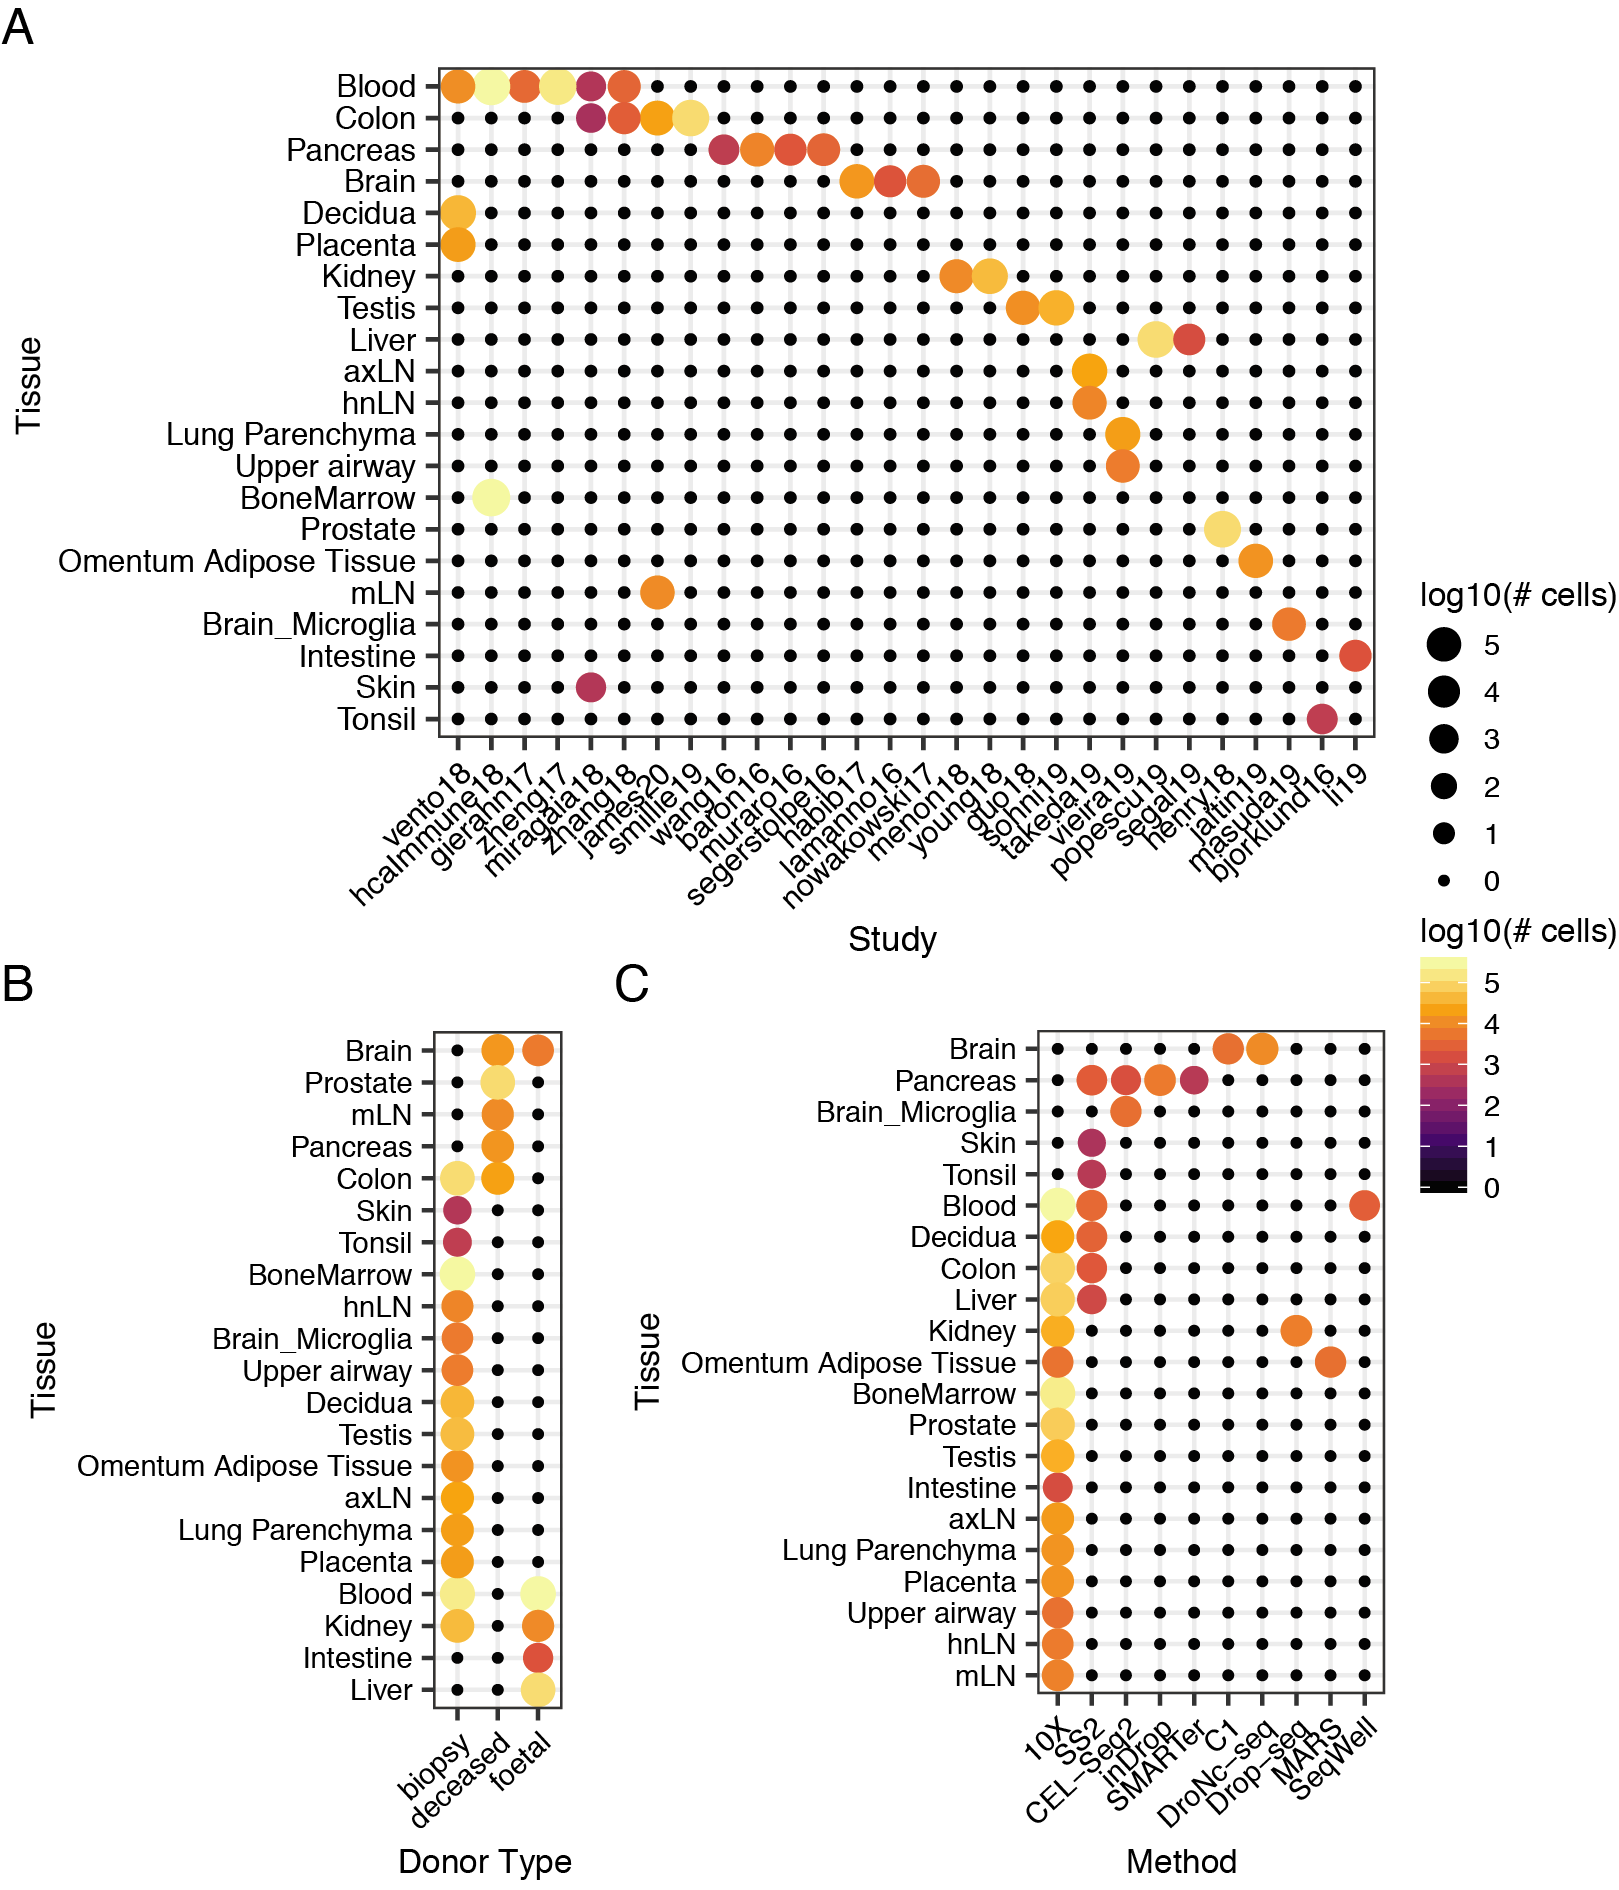
\includegraphics[width=1.0\textwidth]{Chapter4/Figs/chap4_countsHumanAtlas.png} % change word in curlies to change figure
    \caption[Cell numbers in the human dataset collection]{\textbf{Cell numbers in the human dataset collection} \newline Number of cells, in log10 scale, collected from different tissues, and distributed by publication \textbf{(A)}, type of collection \textbf{(B)}, and scRNA-seq protocol \textbf{(C)}.}
    \label{fig:chap4_cha}
\end{figure}

The 28 datasets collected include 21 tissues, mostly collected from adult biopsies (Figure~\ref{fig:chap4_cha}A and ~\ref{fig:chap4_cha}B), and totalling close to 1.5 million cells. Various studies focus on haematopoietic-derived cells, and as such many of the sampled tissues are mostly or completely composed of immune cells. Most cells are obtained using the droplet-based "Chromium" instrument from 10x Genomics ("10X" in Figure~\ref{fig:chap4_cha}C), followed by the plate-based, full-length Smart-seq2 ("SS2"). Despite this unbalance in usage of different technologies, it is in agreement with what has been reported in an exhaustive curated reference of single-cell sequencing datasets~\citep{svensson_curated_2019}.

The collected expression matrices for the listed datasets were combined. Gene references were matched across all datasets (see Methods Section~\ref{section4.4_datacol}). This was done to respect the integrity of each dataset, and facilitate data collection and incorporation (see Section~\ref{section4.3}). The \textit{CellTypist} pipeline was then applied to this collection (see Methods Section~\ref{section4.4_model}), and optimisation resulted in a model with 627 clusters (Figure~\ref{}, Figure~\ref{}A,B), with a classification accuracy of 84\% on left-out test data. For completeness, 3 other models, chosen using different metrics, were also examined (Figure~\ref{}).


\subsection{TBD}
\label{section4.2_test}



\subsection{Gene expression driving cell identity}
\label{section4.2_genes}



\subsection{Matching cell identity across tissues}
\label{section4.2_tissues}



\section{Discussion}
\label{section4.3}
From its inception, the Human Cell Atlas (HCA) consortium has aimed to "define all human cell types in terms of distinctive molecular profiles (such as gene expression profiles)"~\citep{regev_human_2017}. This task is not one that can be easily accomplished by a single team. Beyond the financial and ethical constraints, collecting good quality scRNA-seq data requires tissue-specific knowledge, as well as profiling using both top-down and bottom-up approaches to obtain an overview of cell populations, while capturing cell type-specific phenotypic variations. Yet as data on human cells accumulates, methods capable of compiling the cellular census envisioned by the HCA members, and make it available to the community will be of great use.

% different studies not properly integrated - but can also be that they have many non-overlapping cell types
%% uniform gene reference problems


% use and availability of this data collection
This large human cell type reference can be very useful to the genomics community the relies on single-cell transcriptome profiling to characterise cell identity in a variety of systems. In disease-focused studies, the steady-state reference provided by \textit{CellTypist} can automatically annotate the cells obtained from a disease sample, eliminating the need to obtain a matching healthy sample. Another potential use is to characterise cell fates and heterogeneity when differentiating organoids. Classifying scRNA-seq data from the generated organoids can reveal the cell types present that a specific protocol was able to differentiate. \textit{CellTypist} will also be available as an online resource, where the model can be directly used, and is accompanied by a database showing the defining characteristics of each cell type - marker genes detected, tissues of origin, datasets characterising them, and similar cell types. This is further intended to be articulated with a Cell Ontology~\citep{bard_ontology_2005}, and have cell names be consistently used when new data is produced, with a direct correspondence to both databases.

% bias in collected data
%% model updating with new data will make it more inclusive/glabally applicable
%% over represented cell types might "hide" smaller ones
%% data augmentation/downsampling can help


% gene biology


%tissue biology


\section{Methods}
\label{section4.4}
\subsection{Collecting single-cell expression data}
\label{section4.4_datacol}
Single-cell RNA-seq expression data was collected for the publications listed in Table~\ref{table:tab_4_1}, together with cell type annotations when there were available. Information about tissue, donor type and scRNA-seq protocol were obtained from the publications.

In most cases, count data was available together with the raw sequencing reads in the chosen repository. In other cases, the expression matrices deposited included log normalised data. This means that the data was normalised by the total number of reads/UMI of each cell, often followed by multiplication by a specific scaling factor (usually 10000), and finally log scaled, adding 1 to account for the zeroes present. For these datasets, data was reconverted to counts following an approach similar to that explained in \url{http://www.nxn.se/valent/2018/10/25/unscaling-scaled-counts-in-scrna-seq-data}. Given the scaling factor \textit{S}, representing the second most abundant value for each cell, and \textit{x} for each expression value, unscaled data \textit{U} was obtained by applying Formula 4.1, followed by rounding to the nearest unit to remove floating point inaccuracies.

\begin{align}
U = \frac{\mathrm{e}^{x} - 1}{S}
\end{align}

Raw count matrices were then compiled together, guaranteeing as much correspondence as possible between the diverse gene references used. All gene identifiers were mapped to the corresponding HGNC gene names, and all unique identifiers were kept.


\subsection{\textit{CellTypist} parameter optimisation and training}
\label{section4.4_model}
The \textit{CellTypist} pipeline was applied to the complete human dataset. Data from the same tissues was integrated and clustered using the Leiden algorithm~\citep{traag_louvain_2019} at several resolutions. For tissues with cell type annotations, resolution was optimised using the split-join distance~\citep{dongen_performance_2000} between clusters and cell type annotation, as described in Chapter~\ref{chap:CT_method} Section~\ref{section3.2.1} (Figure~\ref{}).

Following clustering, per tissue logistic regression models were trained, running for 10 epochs of a maximum of 100 iterations each. These models were used to run the cross-tissue cluster merging pipeline (Chapter~\ref{chap:CT_method} Section~\ref{section3.2.2}), and a combination of parameters was chosen based on the ratio of split-join distances (merged vs annotated cell types over per tissue vs annotated cell types) (Figure~\ref{}), resulting in the choice of thr1 = 0.99 and thr2 = 0.8. Additionally, three other combinations were chosen for comparison (Figure~\ref{}): thr1 = 0.4 and thr2 = 0.99, the combination with the top split-join ratio when only considering merged clusters; thr1 = 0.25 and thr2 = 0.25, one of the combinations with the highest fraction of merged clusters; thr1 = 0.1 and thr2 = 0.1, the combination with the highest fraction of merged clusters, as well as highest split-join fraction.

The groupings obtained were used to train a logistic regression model (Chapter~\ref{chap:CT_method} Section~\ref{section3.2.3}) that run for 25 epochs of a maximum of 100 iterations each, using 90\% of the data as a training set, and the remaining as a left out test set that was tested at every iteration (Figure~\ref{}, Figure~\ref{}).


\subsection{Obtaining gene group lists}
\label{section4.4_genelists}
\textit{GO Terms}: GO Terms were downloaded using the biomaRt R package~\citep{durinck_mapping_2009}. Genes from different terms were then grouped in the following categories (similar to~\citep{hagai_gene_2018}): chromatin modulators (GO:0006338 (chromatin remodelling), GO:0003682 (chromatin binding), GO:0042393 (histone binding), and GO:0016568 (chromatin modification)); kinases and phosphatases (GO:0004672 (protein kinase activity) and GO:0004721 (phosphoprotein phosphatase activity)) and catalytic enzymes (GO:0003824 (catalytic activity)).

\textit{Transcription Factors}: Human transcription factors were obtained from AnimalTFDB v3.0 (~\url{http://bioinfo.life.hust.edu.cn/AnimalTFDB/})~\citep{hu_animaltfdb_2019}.

\textit{Housekeeping genes}: Housekeeping genes were obtained from~\url{https://m.tau.ac.il/~elieis/HKG/}~\citep{eisenberg_human_2013}.

\textit{Cell communication-associated genes}: Genes involved in cell-cell communication were obtained from~\url{cellphonedb.org}~\citep{efremova_cellphonedb_2019}.

\textit{Tissue-specific genes}: Tissue specific genes were determined as described in~\citep{sonawane_understanding_2017}. Briefly, RNA-seq expression data from the GTex Consortium was obtained (~\url{https://gtexportal.org/home/index.html})~\citep{consortium_genotype-tissue_2015}, and genes were considered tissue-specific for a given tissue if the difference between their median expression in that tissue and across all tissues normalised by its inter quartile range across all tissues, was greater than 2.


\subsection{Enrichment of gene groups}
\label{section4.4_enr}



